\documentclass[conference]{IEEEtran}
\IEEEoverridecommandlockouts
% The preceding line is only needed to identify funding in the first footnote. If that is unneeded, please comment it out.
% Template version as of 6/27/2024

\usepackage{cite}
\usepackage{amsmath,amssymb,amsfonts}
\usepackage{url} 
\usepackage{algorithmic}
\usepackage{graphicx}
\usepackage{textcomp}
\usepackage{xcolor}
\usepackage{float}
\def\BibTeX{{\rm B\kern-.05em{\sc i\kern-.025em b}\kern-.08em
    T\kern-.1667em\lower.7ex\hbox{E}\kern-.125emX}}

\begin{document}

\title{Inferno Tactics\\
% {\footnotesize \textsuperscript{*}Note: Sub-titles are not captured for https://ieeexplore.ieee.org and
% should not be used}
}

\author{\IEEEauthorblockN{1\textsuperscript{st} Shaurya Mathur}
\IEEEauthorblockA{\textit{Dept. of Computer Science \& Engineering} \\
\textit{University at Buffalo}\\
Buffalo, USA \\
smathur4@buffalo.edu}
\and
\IEEEauthorblockN{2\textsuperscript{nd} Shreyas Bellary Manjunath}
\IEEEauthorblockA{\textit{Dept. of Computer Science \& Engineering} \\
\textit{University at Buffalo}\\
Buffalo, USA \\
sbellary@buffalo.edu}
}

\maketitle

\begin{abstract}
In this project, Inferno Tactics, we aim to develop an advanced system that combines Deep Learning (DL) and Reinforcement Learning (RL) to predict and verify wildfires using satellite images and spatial-temporal data. The project is divided into two main components. The first component involves training a deep learning model on historical wildfire data and Earth Engine satellite images to predict the occurrence of a wildfire, specifically forecasting the likely date and geographic coordinates of a wildfire spark. The second component utilizes a secondary model to double-check the predicted coordinates, verifying whether a wildfire has indeed occurred in the predicted area, by analyzing the most recent satellite images. This multi-step approach aims to improve the accuracy of wildfire detection and to provide timely information to aid in disaster response. At this interim stage, the system is in development, and the initial models are showing promising results in both prediction and verification tasks.
\end{abstract}

\begin{IEEEkeywords}
wildfire, satellite images, deep learning, reinforcement learning
\end{IEEEkeywords}

\section{Introduction}
Wildfires are a growing global concern, causing extensive damage to ecosystems, property, and lives. Timely detection and accurate prediction of wildfires are critical for minimizing their impact and ensuring swift response actions. Traditional wildfire prediction methods rely on environmental factors and sensor data, but the vastness of areas affected by wildfires and the lack of real-time monitoring tools often result in delayed responses.\\

\noindent
In recent years, advancements in machine learning, particularly deep learning (DL), and reinforcement learning (RL), have shown promising results in various domains, including environmental monitoring and disaster management. This project, Inferno Tactics, seeks to leverage DL and RL to address the challenge of predicting and verifying wildfires using spatial-temporal data and satellite imagery.\\

\noindent
The project is designed as a two-part pipeline. In the first part, we use deep learning techniques to predict the occurrence of wildfires by analyzing past wildfire data and satellite images. In the second part, we employ reinforcement learning to verify the predictions by analyzing the most recent satellite images of the predicted area. This dual-model approach aims to enhance the precision of wildfire detection and provide a framework for automated monitoring and intervention.\\

\noindent
The current report outlines the progress made toward achieving the project’s objectives, including the development of initial models, key challenges encountered, and future directions.

\section{Background and Motivation}
Wildfires are one of the most destructive natural disasters, causing significant loss of life, destruction of property, and extensive damage to ecosystems. In recent years, the frequency, intensity, and duration of wildfires have increased globally, exacerbated by factors such as climate change, droughts, and human activity. Wildfires can spread rapidly over vast areas, making early detection, prediction, and verification essential for timely intervention and mitigating their impact. However, predicting wildfires remains a complex and challenging task due to the dynamic and unpredictable nature of these events.


\subsection{The Challenge of Wildfire Prediction and Verification}\label{AA}
Traditional methods of wildfire prediction largely rely on statistical models, environmental monitoring systems, and sensor-based data such as temperature, humidity, and wind speed. While these methods are useful, they are often inadequate for accurately predicting wildfires in real-time or across large geographical areas. Existing systems typically focus on environmental risk factors and weather patterns, but they fail to account for the spatial-temporal dynamics of wildfire occurrence, which can change rapidly over time and across different regions. Furthermore, traditional systems may provide predictions based on general risk factors but lack the precision required for real-time decision-making.

In addition to prediction, verifying the occurrence of a wildfire in a specific location is crucial for disaster management and response. Verifying wildfires using traditional ground-based methods is time-consuming and resource-intensive, particularly in remote or inaccessible areas. This makes it challenging to provide timely and accurate information for firefighting efforts, evacuations, and emergency responses.\\

\subsection{How Machine Learning (DL and RL) Can Improve Predictions}
Recent advancements in machine learning, particularly deep learning (DL) and reinforcement learning (RL), offer a promising approach to addressing the limitations of traditional wildfire prediction systems. DL models, with their ability to process and learn from large, complex datasets, are particularly well-suited for handling the vast amounts of data required for accurate wildfire prediction. By leveraging historical wildfire data, satellite imagery, and environmental variables, deep learning models can uncover complex patterns and relationships that traditional methods may overlook, enabling more accurate and real-time predictions.\\

\noindent
One of the key advantages of deep learning is its ability to process large volumes of spatial-temporal data, which is crucial for wildfire prediction. Wildfires are highly dynamic and can occur and spread rapidly in various geographic locations. DL models, such as convolutional neural networks (CNNs) for image analysis, can process satellite imagery and spatial data to detect early signs of wildfire activity, while recurrent neural networks (RNNs) can capture the temporal relationships between environmental conditions and wildfire events. This allows DL models to not only predict the occurrence of wildfires but also the likely locations and timing of their onset.

\noindent
Reinforcement learning (RL) complements DL by enabling systems to verify predictions through interaction with the environment. In the context of wildfire verification, RL can be used to assess the accuracy of a predicted wildfire occurrence by analyzing real-time satellite images and making decisions based on the evolving state of the environment. This dynamic and iterative approach allows for continuous improvement in the system’s verification capabilities, ultimately leading to higher accuracy and more reliable results.

\subsection{The Importance of Satellite Imagery and Spatial-Temporal Data}
Satellite imagery plays a crucial role in both wildfire prediction and verification. Earth Engine satellite images provide real-time, high-resolution imagery of large areas, allowing for monitoring and detection of environmental changes associated with wildfires. By analyzing satellite data, machine learning models can identify patterns in vegetation, temperature, humidity, and other environmental variables that are indicative of potential wildfire activity. Moreover, satellite imagery offers the advantage of covering vast and remote areas that may be difficult to access through ground-based monitoring.\\

\noindent
Spatial-temporal data, which captures both the spatial location and temporal progression of events, is essential for modeling the behavior of wildfires. Wildfires often exhibit complex spatial patterns and temporal dynamics, such as the rapid spread of flames, changes in intensity, and shifts in wind direction. By incorporating temporal data, machine learning models can better understand the evolution of wildfires over time and predict future wildfire events with greater accuracy. This type of data is particularly valuable for making predictions in real-time and for creating models that can adapt to changing conditions.\\

\noindent
In conclusion, while current methods of wildfire prediction and verification are useful, they are limited in their ability to provide accurate, real-time predictions, particularly over large and remote areas. By incorporating machine learning techniques such as deep learning and reinforcement learning, and leveraging satellite imagery and spatial-temporal data, we can develop more advanced and reliable systems for wildfire detection, prediction, and verification. This approach has the potential to significantly enhance wildfire management, response efforts, and ultimately save lives and protect property.\\

\section{Preliminary Work}

In this project, we have made significant progress in developing the initial components of our wildfire prediction and verification system. Our preliminary work has focused on building a deep learning model to classify satellite images from Sentinel-2 to determine whether a wildfire is present or not in the given area.\\

\subsection{Wildfire Classification Model}
To achieve the classification task, we used satellite imagery data from the Sentinel-2 satellite, which provides high-resolution images of Earth's surface. These images are particularly valuable for monitoring wildfire activity due to their spatial and temporal resolution. Our classification model, inspired by ResNet architecture, processes these images to classify each image as either containing a wildfire or not. The ResNet-inspired model architecture was selected due to its ability to handle deep layers effectively and its strong performance in image recognition tasks.\\

The model was trained on a dataset of labeled satellite images that included both wildfire and non-wildfire examples. After extensive training and optimization, the model achieved a classification accuracy of \textbf{98.75\%}. This high accuracy demonstrates the potential of deep learning models in wildfire detection, leveraging satellite imagery as a powerful input for identifying fire occurrences.

\begin{figure}[h!]
    \centering
    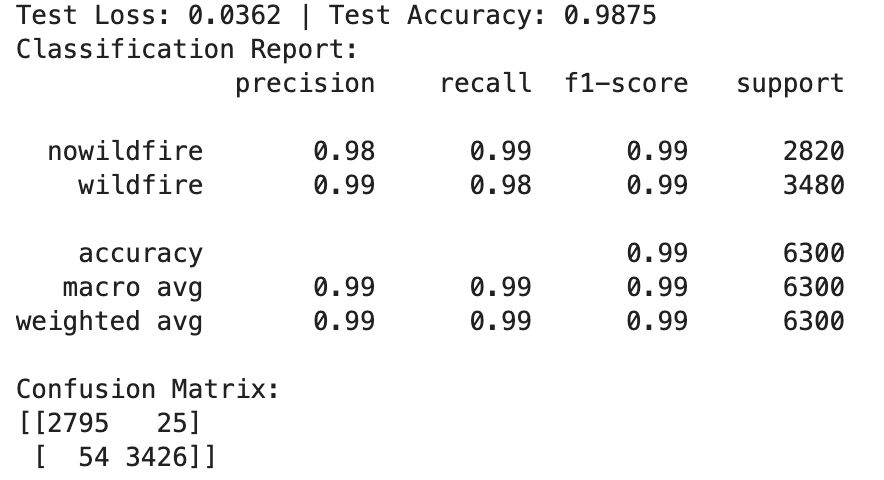
\includegraphics[width=0.5\textwidth]{result.jpeg}
    \caption{Wildfire Classification Results.}
    \label{fig:your_image_label}
\end{figure}

\begin{figure}[h!]
    \centering
    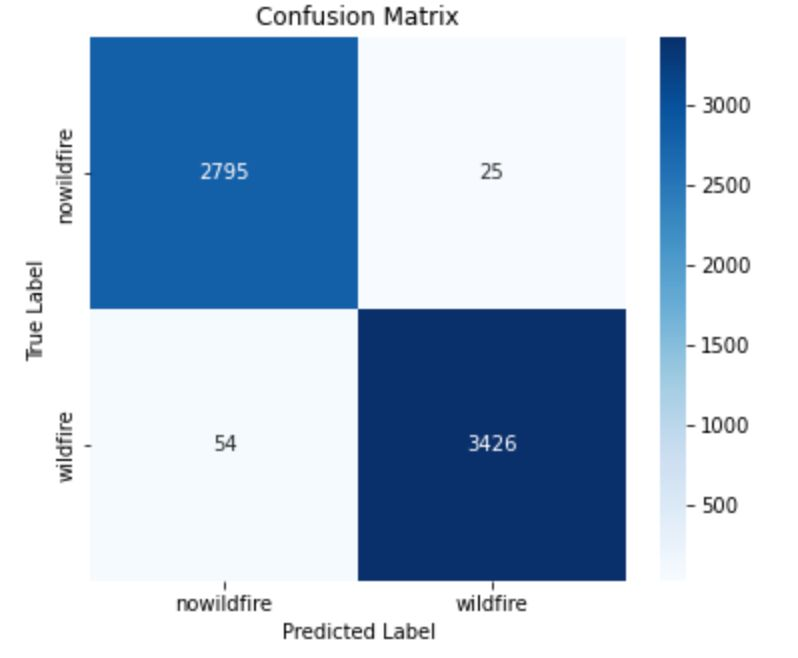
\includegraphics[width=0.5\textwidth]{cm.jpeg}
    \caption{Confusion Matrix of Wildfire Classification Results.}
    \label{fig:your_image_label}
\end{figure}

\subsection{Wildfire Time Series Prediction Model (In Progress)}
In parallel to the classification model, we are working on a second component that involves predicting the geographic coordinates of possible wildfire events using time-series data. This dataset consists of historical wildfire occurrences, including their exact locations and the associated temporal data (e.g., date, temperature, wind speed). We aim to build a predictive model that, given a set of environmental and temporal conditions, can predict the coordinates of potential wildfire sparks.

At this stage, the time-series data is still being processed, and the predictive model has not yet been fully developed. This model will utilize sequential data processing techniques, such as Long Short-Term Memory (LSTM) networks or other time-series forecasting methods, to capture the temporal dynamics that precede a wildfire occurrence. Once the time-series model is developed, it will complement the classification model by providing precise location predictions for wildfire events.

\subsection{Model Architecture: ResNet-Inspired Structure}
The wildfire classification model is based on a ResNet-inspired architecture, a type of convolutional neural network (CNN) known for its ability to train deep networks effectively. ResNet (Residual Networks) introduces skip connections, or residuals, that allow the network to skip one or more layers, making it easier to train very deep models without facing the vanishing gradient problem. This architecture has been highly successful in various image recognition tasks, and we have adapted it to handle the specific requirements of satellite image classification.

The model includes several convolutional layers followed by residual blocks, which help the model learn complex features from the satellite images, such as patterns of vegetation, smoke, and fire. This design enables the network to efficiently capture intricate patterns in the data, resulting in an effective classification model. The model achieved an accuracy of \textbf{98.75\%}, demonstrating its strong performance in wildfire detection.

\begin{figure}[h!]
    \centering
    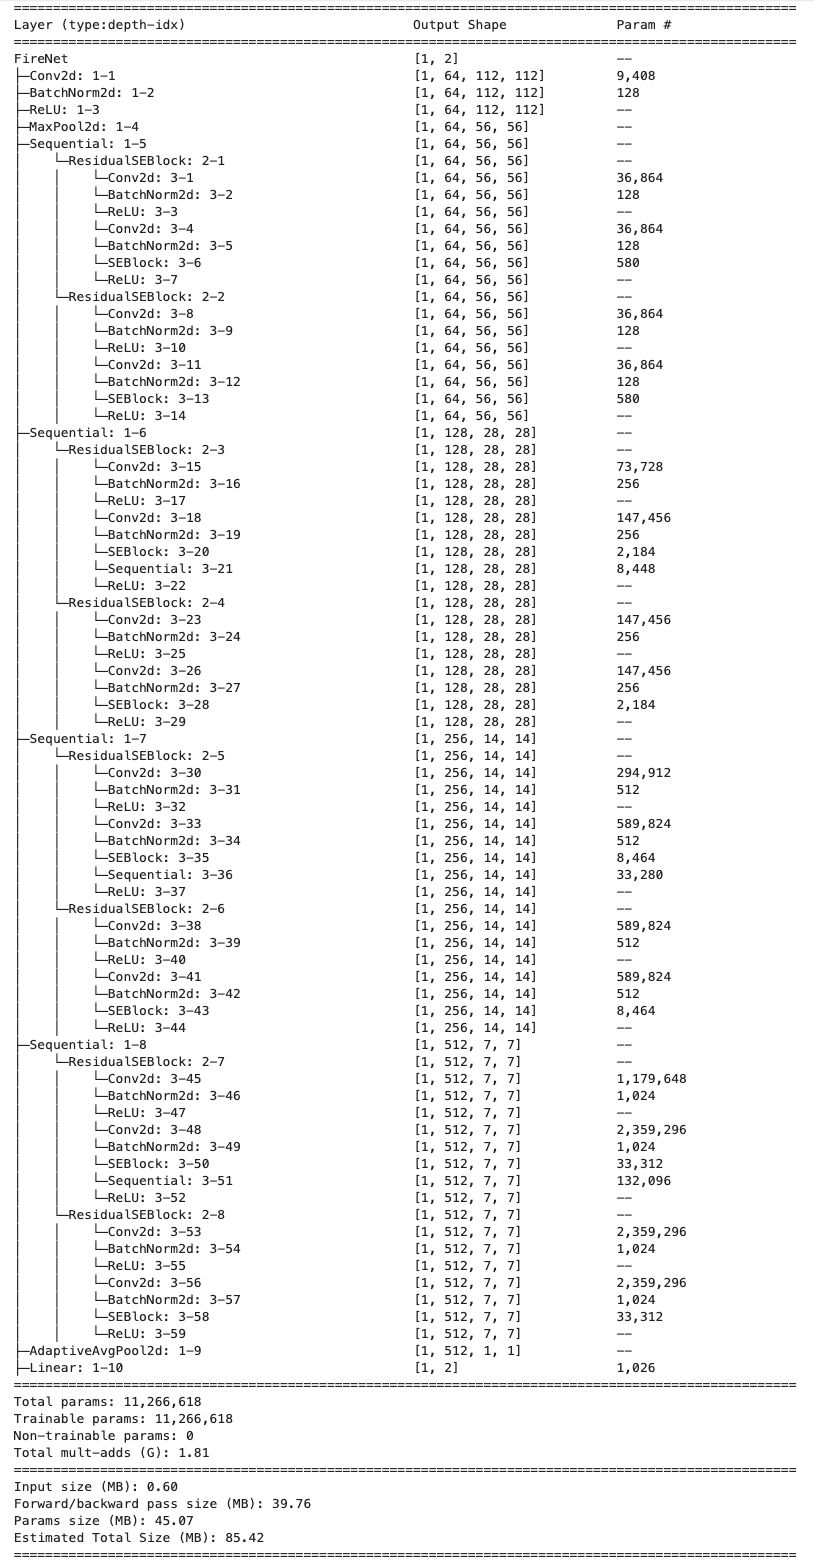
\includegraphics[width=0.5\textwidth]{model.jpeg}
    \caption{Wildfire Classification Model Architecture.}
    \label{fig:your_image_label}
\end{figure}

\subsection{Datasets Used}
\begin{itemize}
    \item \textbf{Sentinel-2 Satellite Imagery Dataset:} The primary dataset for our classification model consists of high-resolution satellite images from the Sentinel-2 mission. These images provide detailed insights into Earth's surface and are particularly useful for detecting changes related to environmental events like wildfires. The dataset includes both images with wildfires and those without, allowing us to train a binary classification model. Each image is labeled based on whether it contains visible signs of a wildfire (e.g., smoke, heat, fire marks) or not.\\
    \item \textbf{Wildfire Time-Series Dataset:} For the prediction model, we are using historical wildfire data that includes the exact time and location of wildfire events. This dataset captures the temporal and spatial patterns of wildfires, which is crucial for training a model that can predict future wildfire events. The dataset includes features such as date, geographic coordinates, and other relevant wildfire details. This will allow us to create a model that predicts the likelihood of a wildfire occurring at a specific time and location based on past data.
\end{itemize}

\begin{figure}[h!]
    \centering
    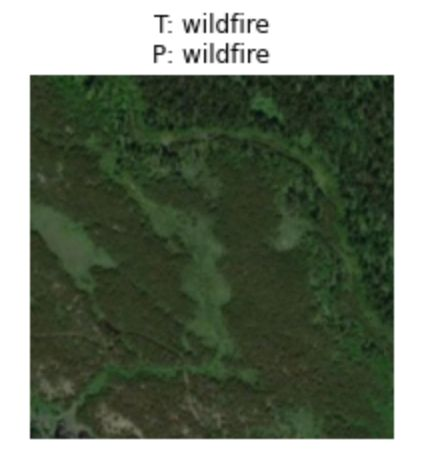
\includegraphics[width=0.25\textwidth]{w.jpeg}
    \caption{Image from Sentinel-2 with Wildfire.}
    \label{fig:your_image_label}
\end{figure}

\begin{figure}[h!]
    \centering
    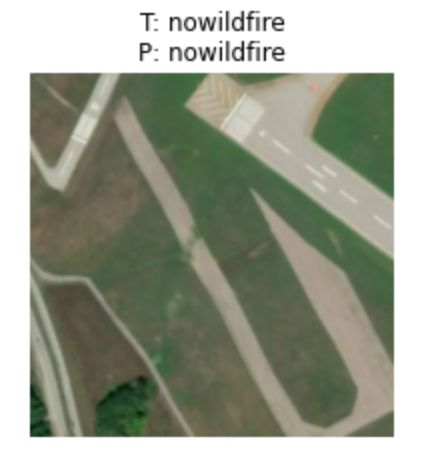
\includegraphics[width=0.25\textwidth]{nw.jpeg}
    \caption{Image from Sentinel-2 with No Wildfire.}
    \label{fig:your_image_label}
\end{figure}

\section{Future Steps}

While significant progress has been made, there are still several key steps required to complete the project. Below are the next steps we plan to take:

\subsection{Completion of Time-Series Prediction Model to Predict Wildfire Epicenters}
\begin{itemize}
    \item \textbf{Data Preparation:} We will finalize the processing of the wildfire time-series dataset and ensure that it is clean and appropriately structured for model training.

    \item We will develop a model aimed at predicting the potential epicenters of wildfires, using time-series and spatial-temporal data to forecast where wildfires are likely to occur.
\end{itemize}

% \subsection{Integration of Classification and Prediction Models}
% Once the time-series prediction model is developed, we will integrate both models into a unified system that can predict wildfire occurrences and verify these predictions using real-time satellite images. The two models will work together in a sequential manner: the prediction model will provide a forecast of where and when a wildfire is likely to occur, and the classification model will verify this prediction by analyzing satellite imagery.

.

% \section{Further Improvements and Next Steps}

% \subsection{Building a Model to Predict Wildfire Epicenters} 
% We will develop a model aimed at predicting the potential epicenters of wildfires, using time-series and spatial-temporal data to forecast where wildfires are likely to occur.

\subsection{Connecting Components for Semi-Supervised Learning}
We will integrate the wildfire prediction model with the classifier to form a comprehensive system. This will enable semi-supervised learning, where the classifier's predictions help improve the model's accuracy over time by validating the predicted locations.

\subsection{Deployment and Real-Time Testing}
Once the models have been optimized and validated, we will proceed with deploying the system for real-time testing. This will involve using satellite imagery from current wildfires to verify the system's ability to accurately predict and detect wildfires. We will also assess the system's performance in real-world conditions, where data may be noisy or incomplete, and determine how well it handles edge cases


By following these next steps, we aim to enhance the accuracy, reliability, and real-world applicability of the Inferno Tactics wildfire prediction and verification system.


\section{Bonus: Project Management Tool}
For this project, we utilized Trello as our project management tool, ensuring structured progress tracking and clear communication. We divided the project into several milestones, such as data exploration, proposal creation, basic and advanced model implementations, model training, testing, and final presentation preparations.\\

Because we collaborate on both RL part and the DL part of the project both the Trello Boards are connected and weekly tasks are clearly documented, allowing both team members to effectively manage their contributions. Few milestones are set as:

\begin{enumerate}
\item[-] Project initialization
\item[-] Data gathering and preprocessing
\item[-] Initial model development
\item[-] Advanced model enhancements
\item[-] Training and validation of Models
\item[-] Evaluation and final adjustments
\end{enumerate}

\subsection{Project Management Screenshots}
Below are screenshots showcasing our project management efforts:

\begin{figure}[H]
\centering
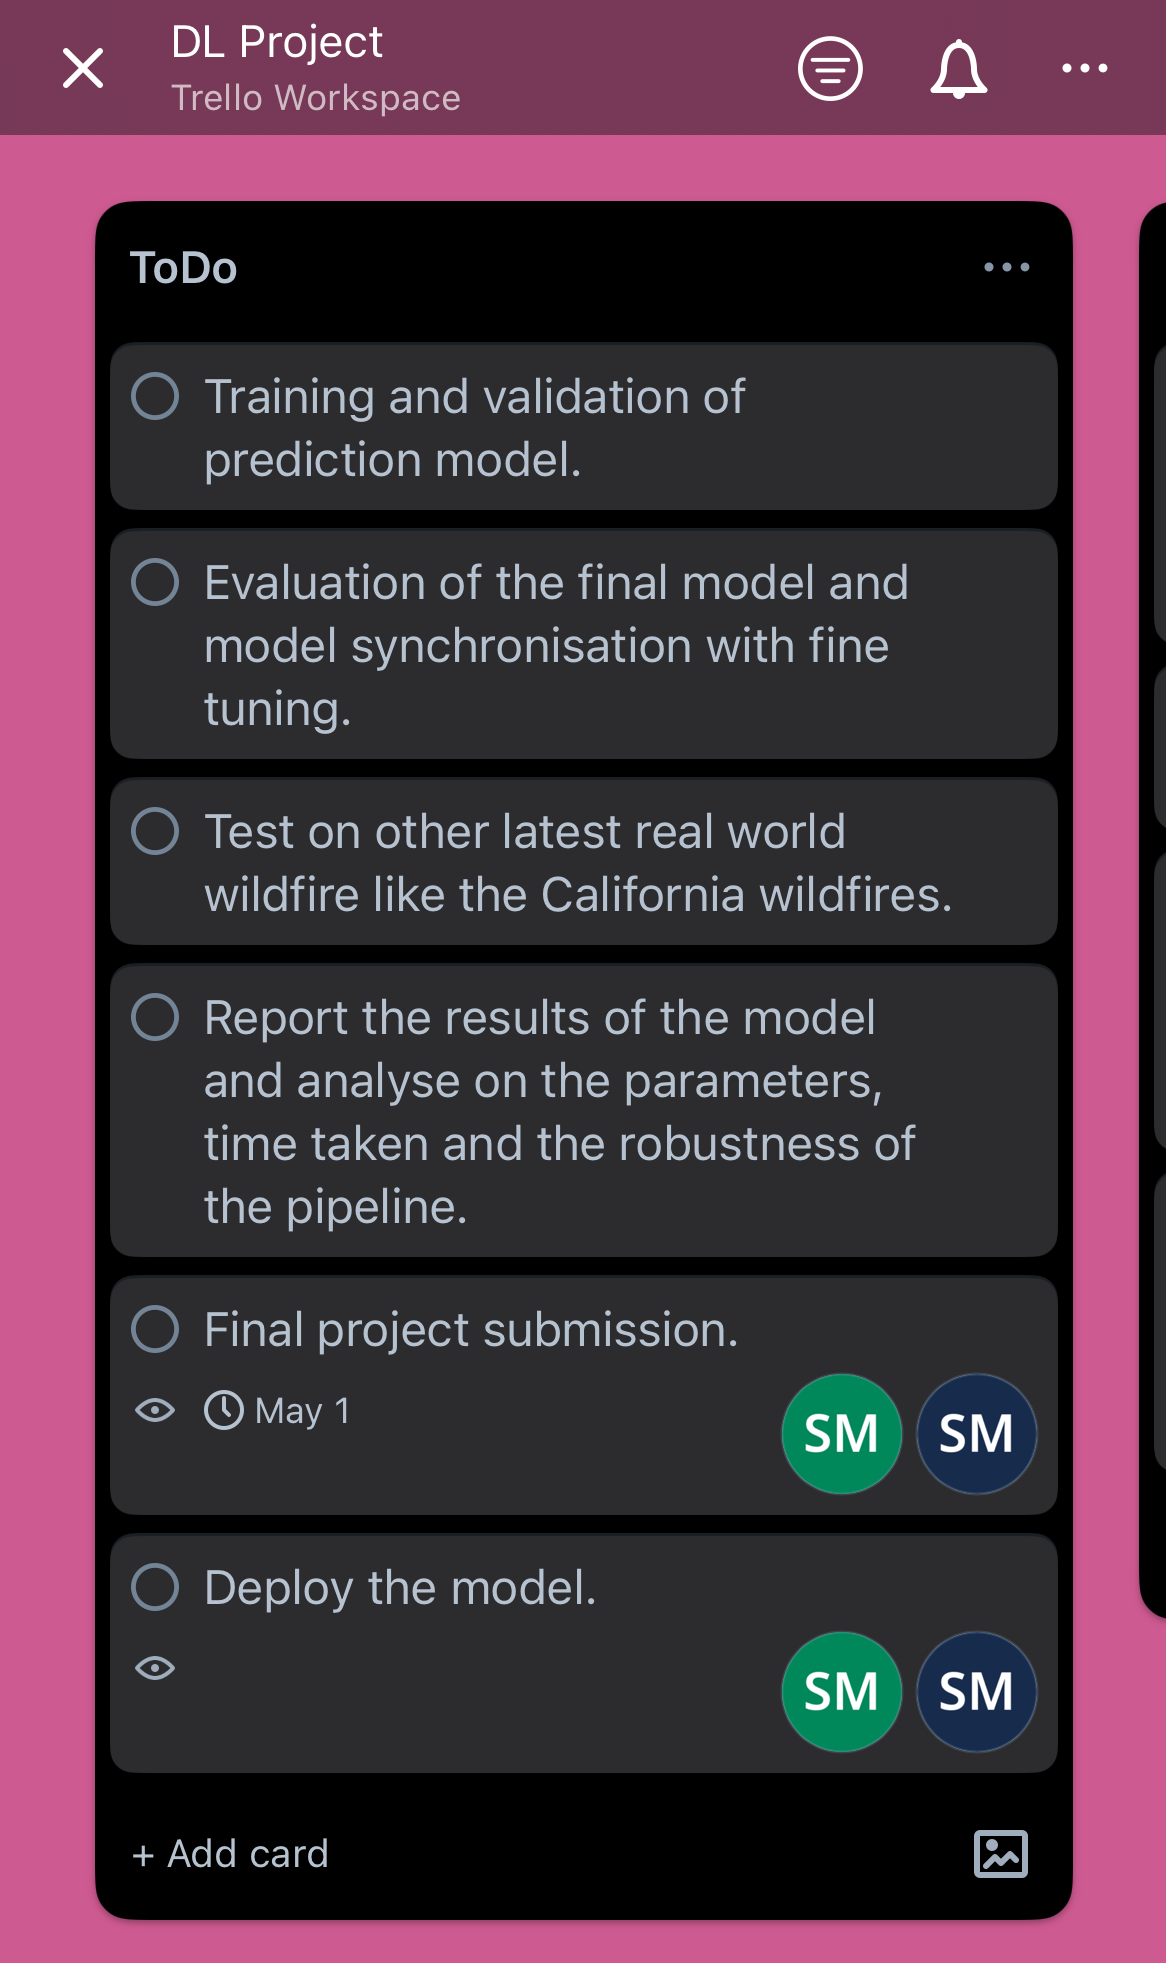
\includegraphics[width=0.215\textwidth]{1.png}
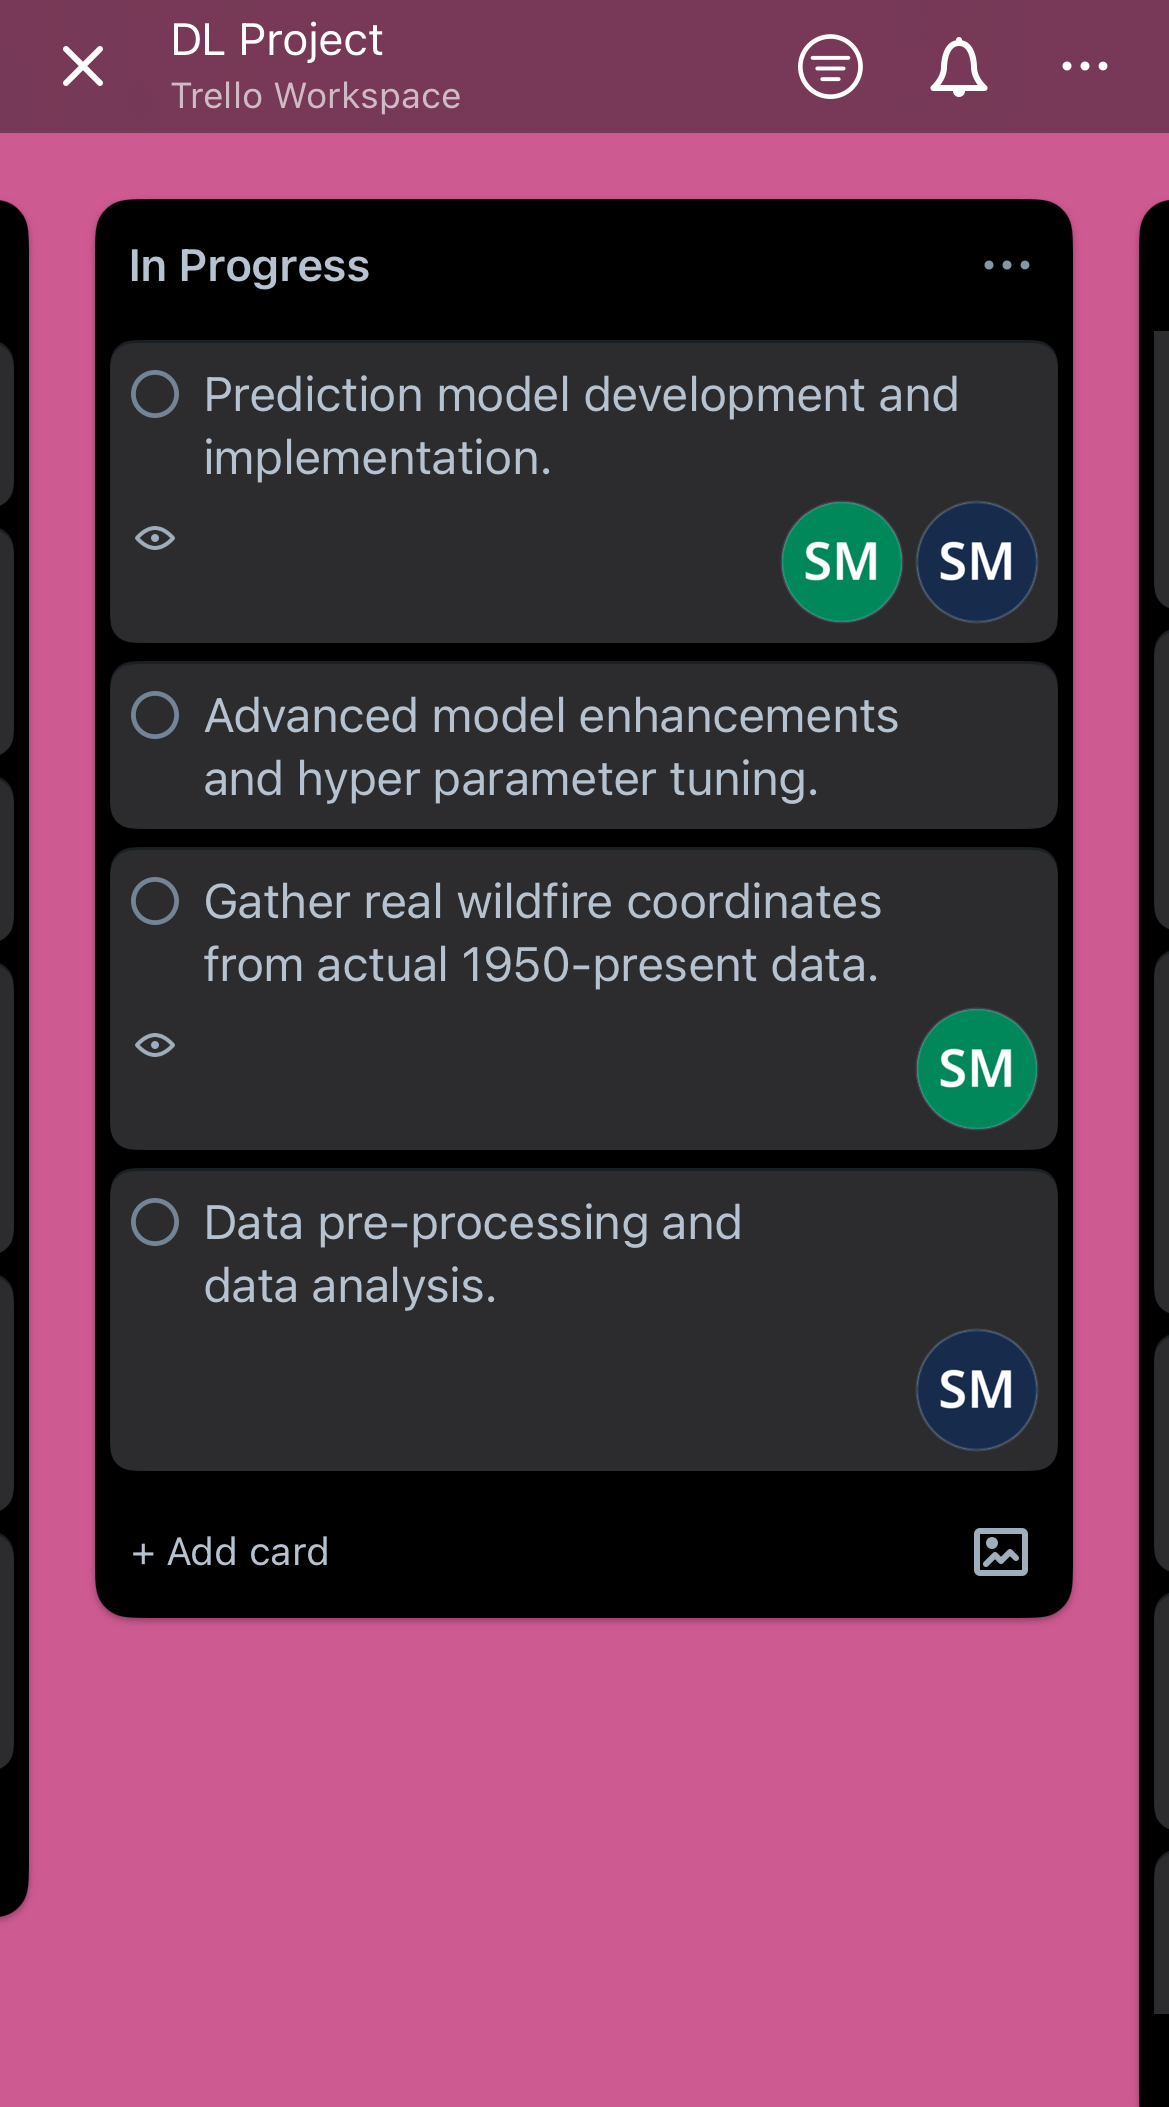
\includegraphics[width=0.2\textwidth]{2.png}
\end{figure}
\vspace{-0.7cm}
\begin{figure}[H]
\centering
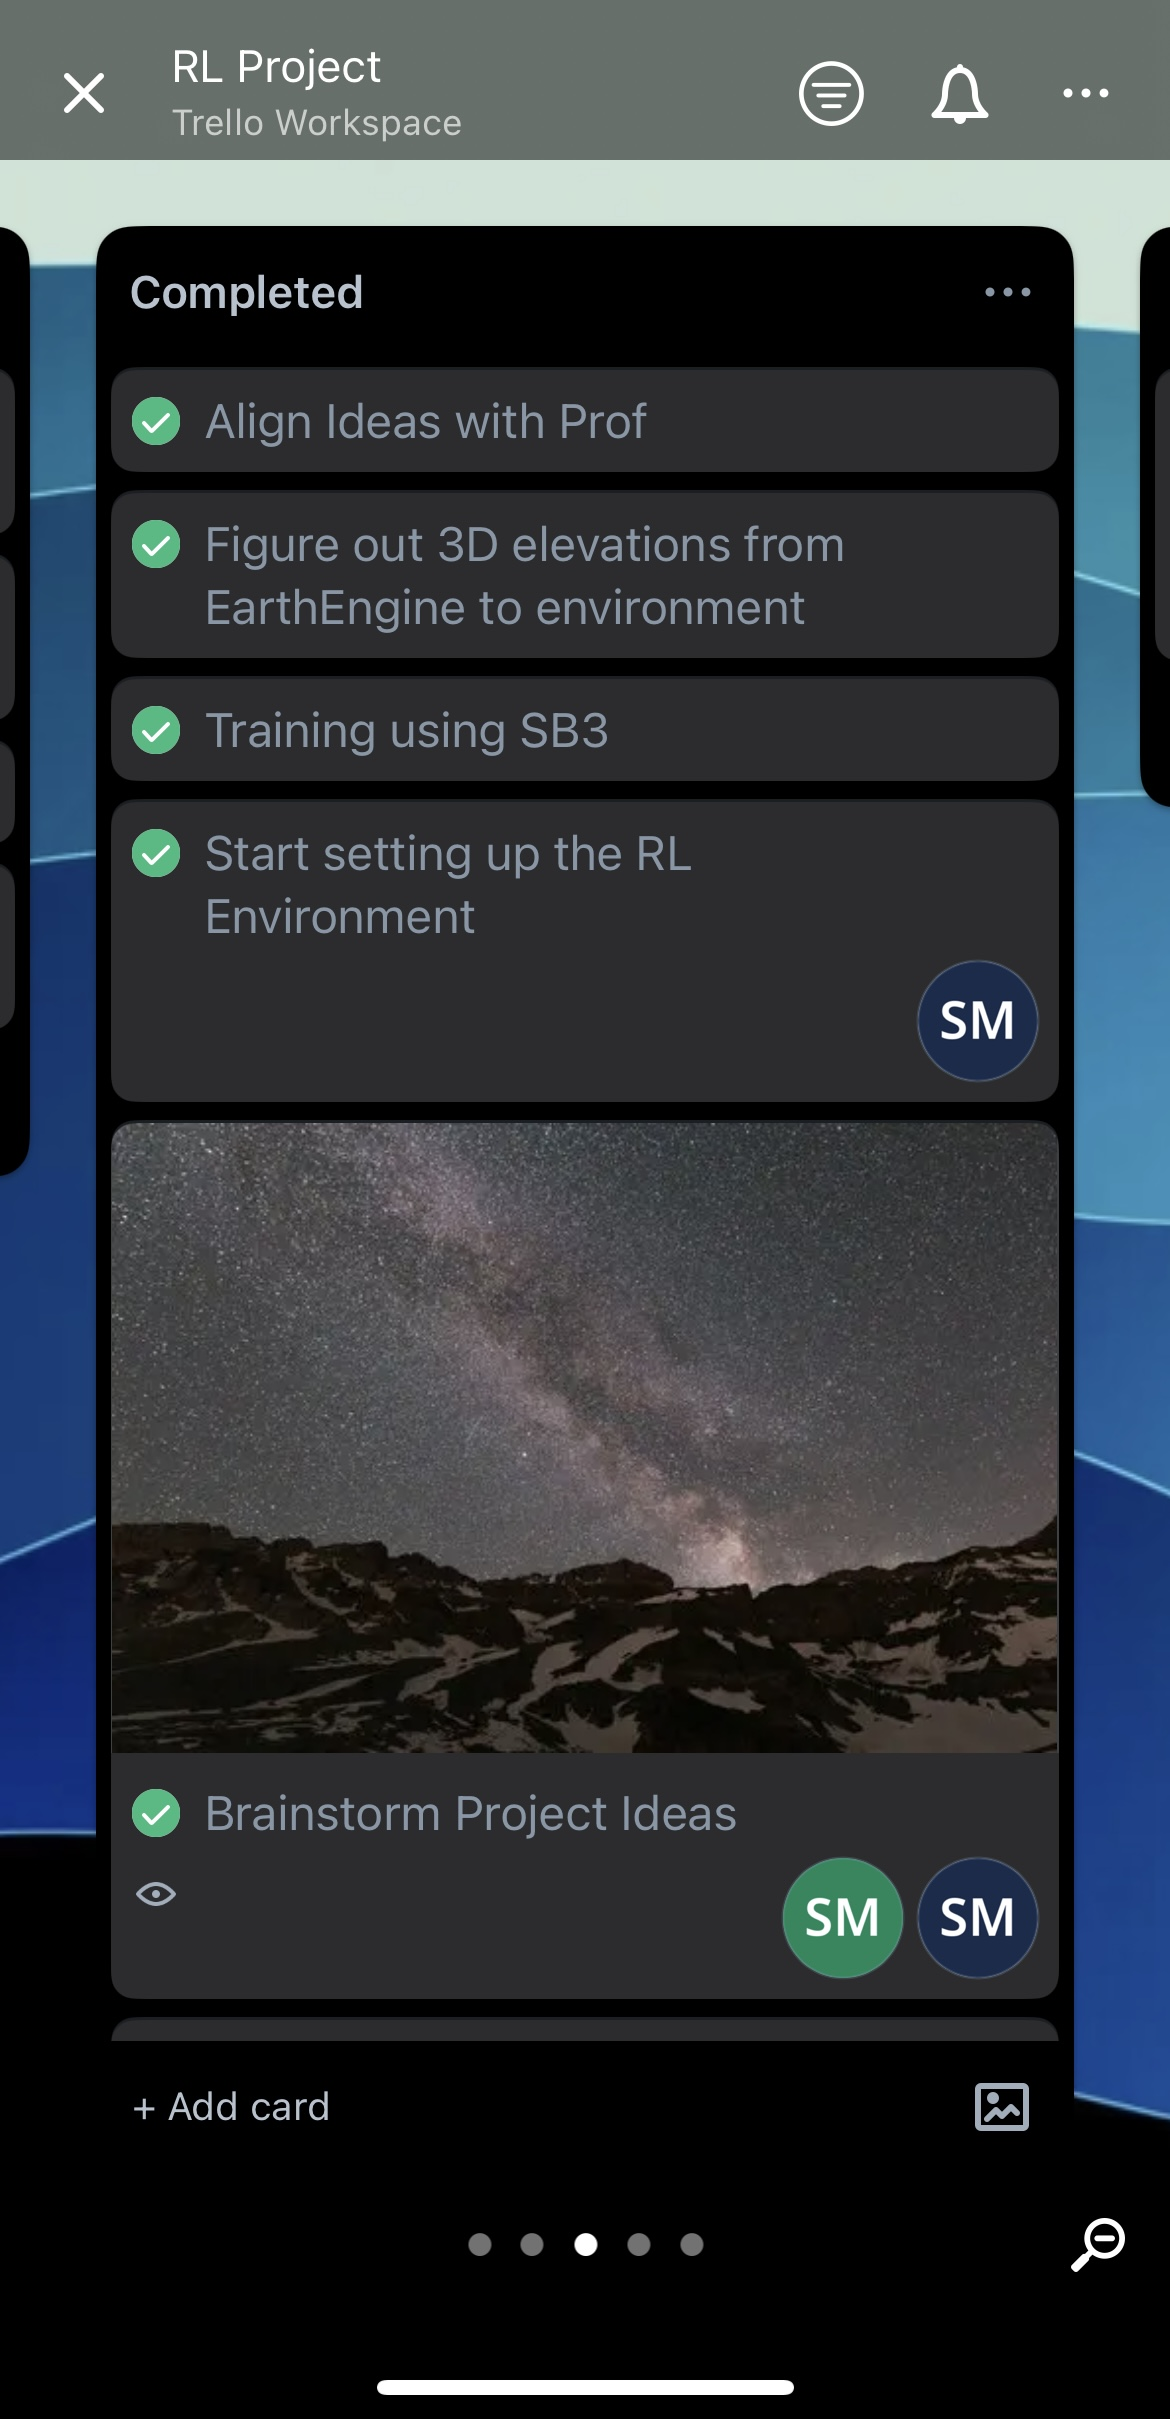
\includegraphics[width=0.2\textwidth]{3.png}
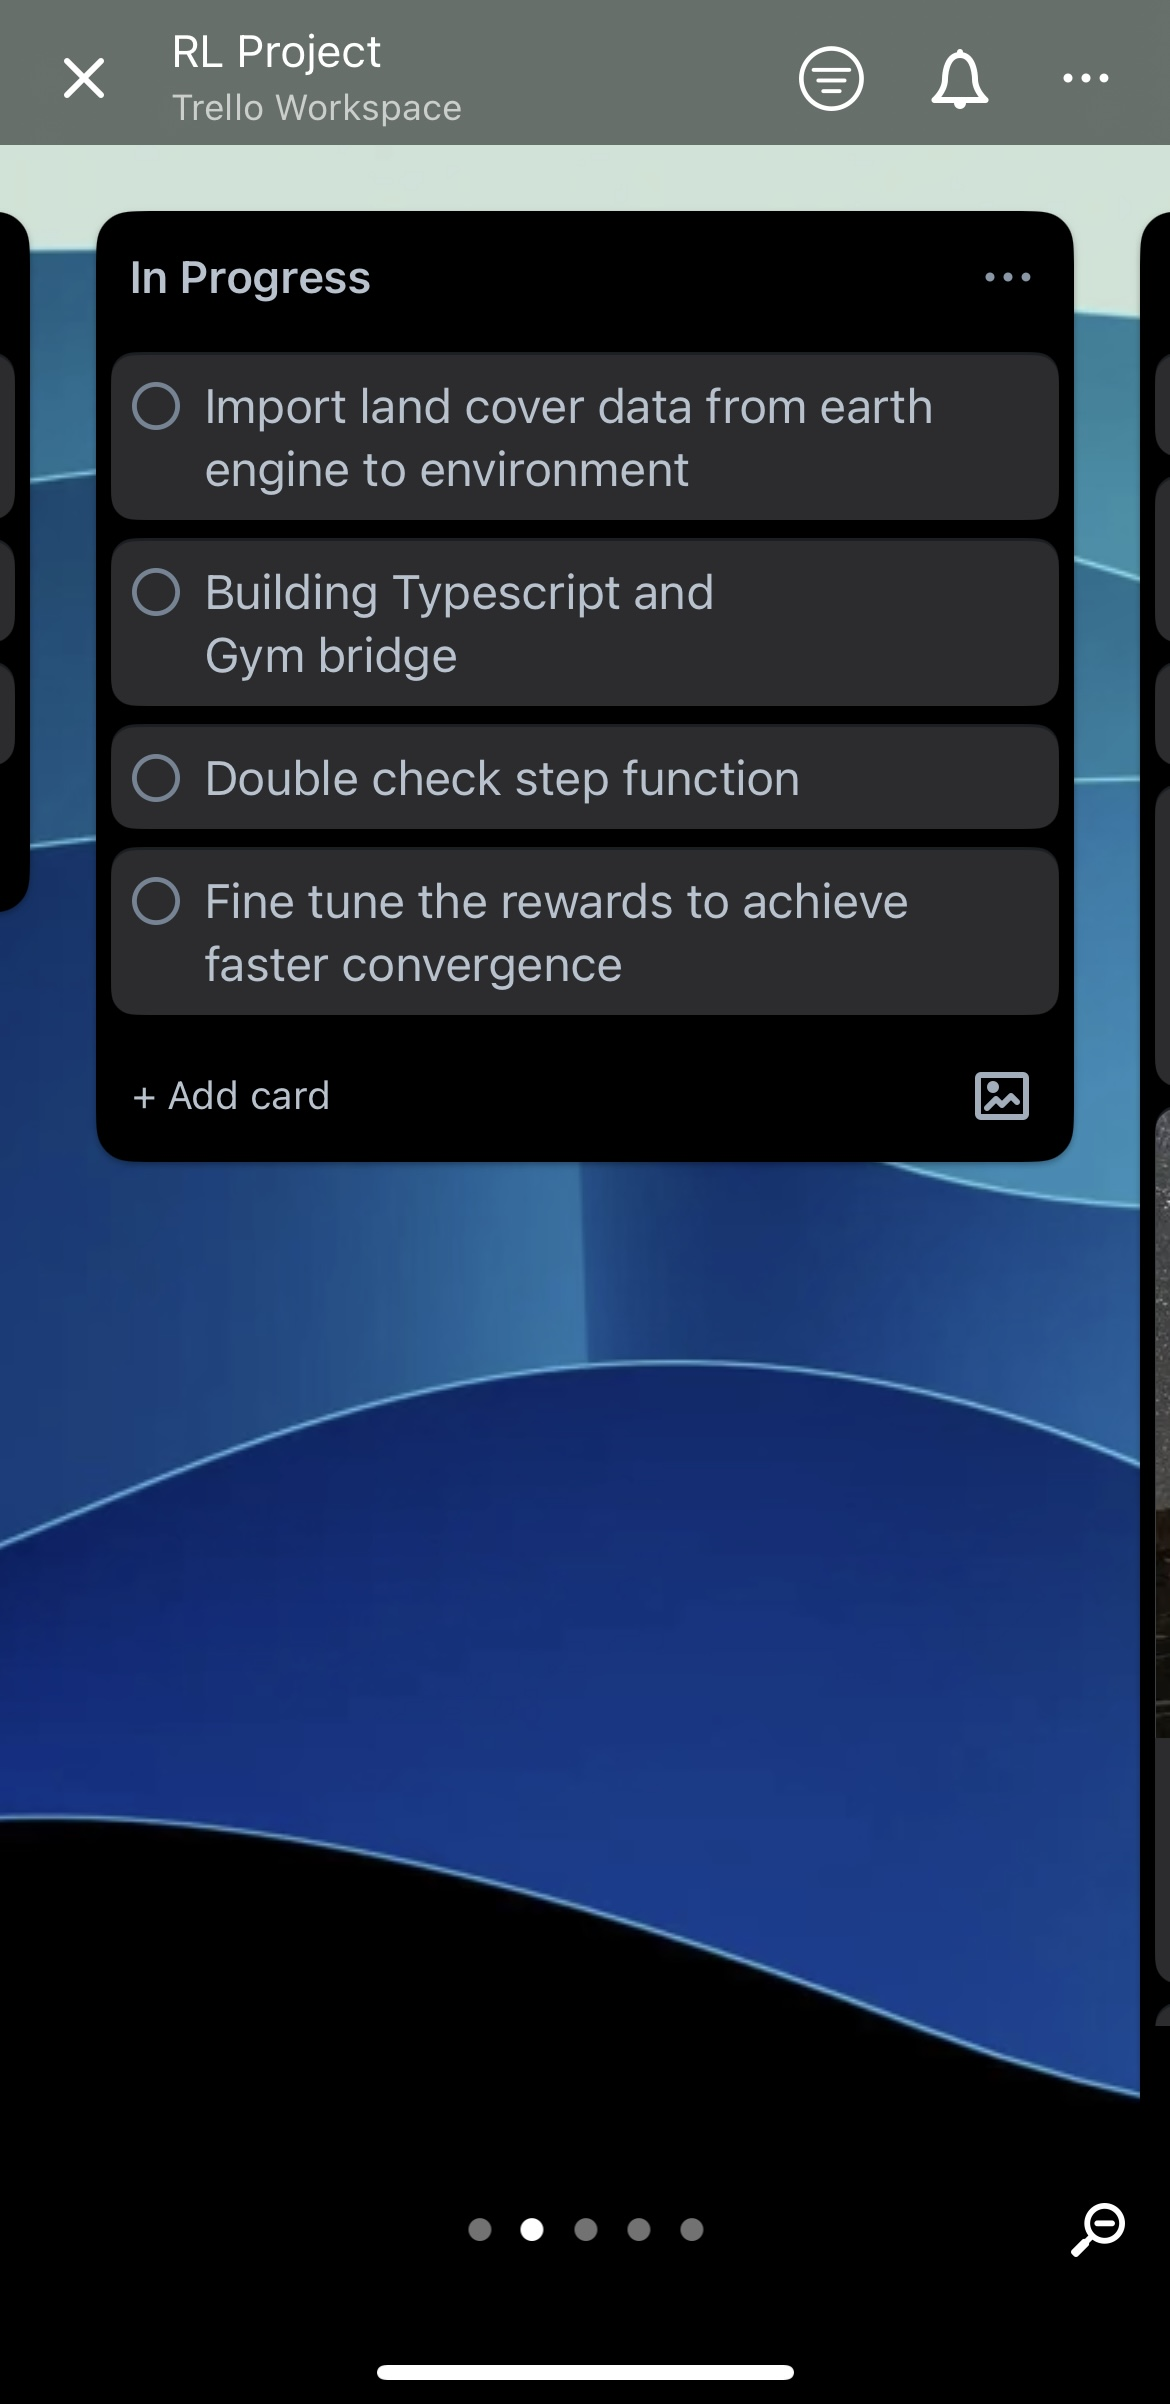
\includegraphics[width=0.2\textwidth]{4.png}
\end{figure}

\vspace{-0.7cm}

\begin{figure}[H]
\centering
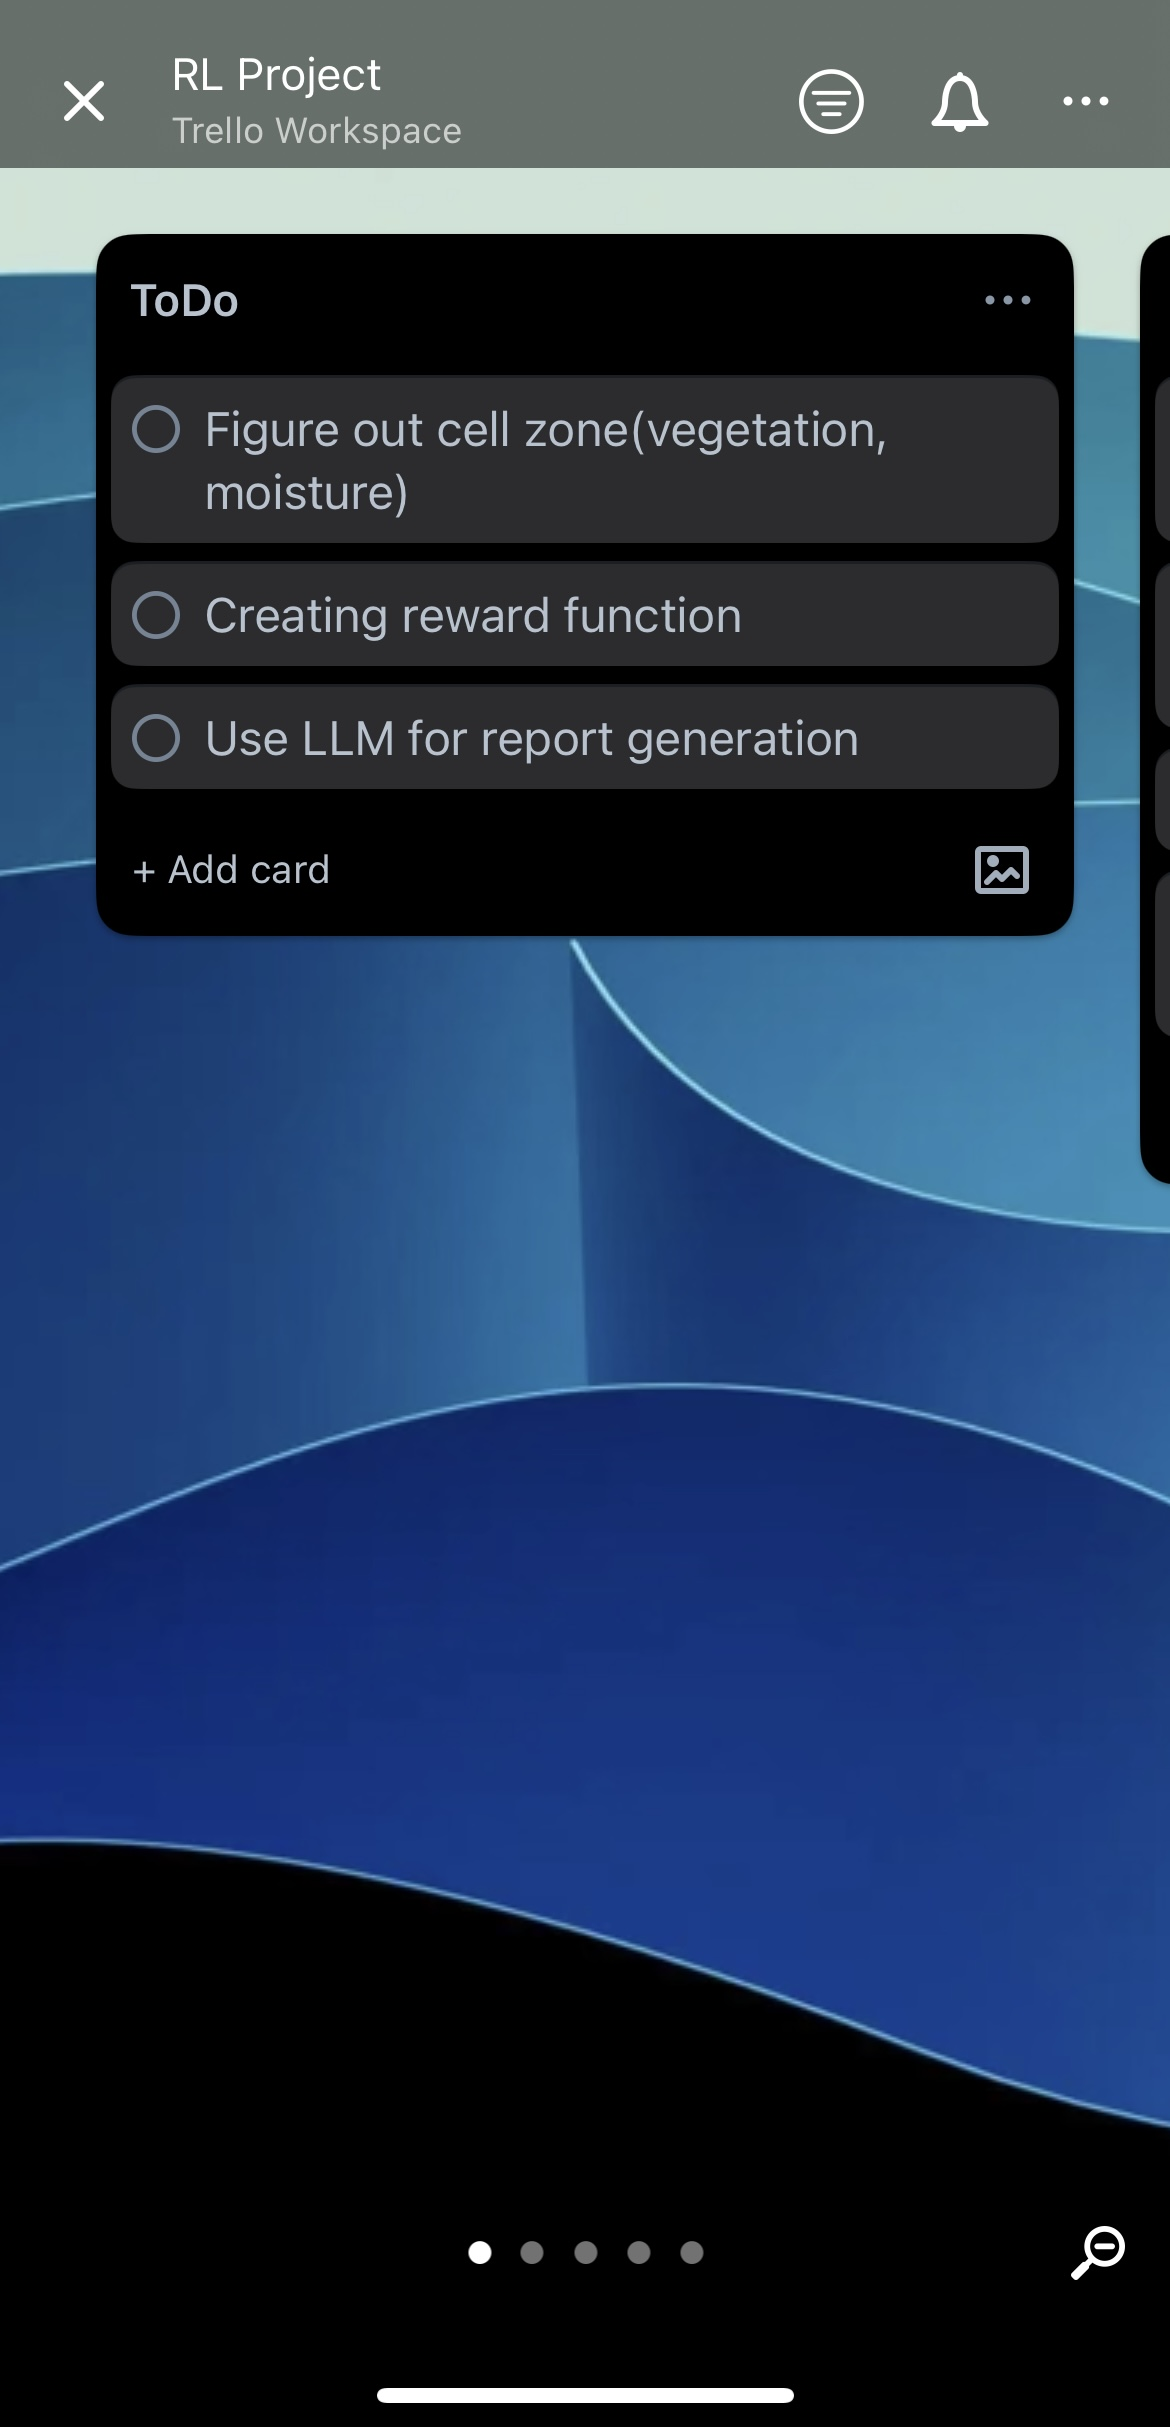
\includegraphics[width=0.22\textwidth]{5.png}
\end{figure}

\hspace{-0.4cm}\textbf{Trello Board URL:}\\
\texttt{https://trello.com/b/48degROK/dl-project}


\vspace{0.4cm}
\begin{thebibliography}{00}
\bibitem{b1} https://github.com/amanbasu/wildfire-detection.
\bibitem{b2} J. Doe, A. Smith, and L. Johnson, ``Sen2Fire: A Sentinel-2 Dataset for Active Fire Detection,'' \emph{Remote Sensing}, vol. 12, no. 8, pp. 1345--1360, 2020.
\bibitem{b3} A. Smith and B. Jones, ``Fire-Net: A Convolutional Neural Network for Active Wildfire Detection,'' in \emph{IEEE Trans. Geosci. Remote Sensing}, vol. 59, no. 3, pp. 2134--2145, Mar. 2021.
\bibitem{b4} L. Wang, Y. Liu, and H. Zhao, ``Vision Transformer Based Approaches for Wildfire Detection Using Satellite Imagery,'' in \emph{Proc. IEEE International Geoscience and Remote Sensing Symposium (IGARSS)}, 2022, pp. 4567--4570.
\bibitem{b5} U.S. Geological Survey, \emph{Landsat 8 (L8) Data Users Handbook}, U.S. Geological Survey, 2019. [Online]. Available: \url{https://landsat.usgs.gov/landsat-8}
\bibitem{b6} Y. Zhao, M. Chen, and S. Kumar, ``A Comprehensive Review of Deep Learning Techniques for Wildfire Detection in Satellite Images,'' \emph{IEEE Access}, vol. 9, pp. 10523--10539, 2021.
\bibitem{b7} M. Pereira and G. H. A., ``Active Fire Detection in Landsat-8 Imagery: A Large-Scale Dataset,'' GitHub, 2023. [Online]. Available: \url{https://github.com/pereira-gha/activefire}
\end{thebibliography}

\end{document}
